\newpage
\section{Transient Absorption Spectroscopy}
\label{sec:transientTheory}

\begin{center}
    \captionsetup{type = figure}
    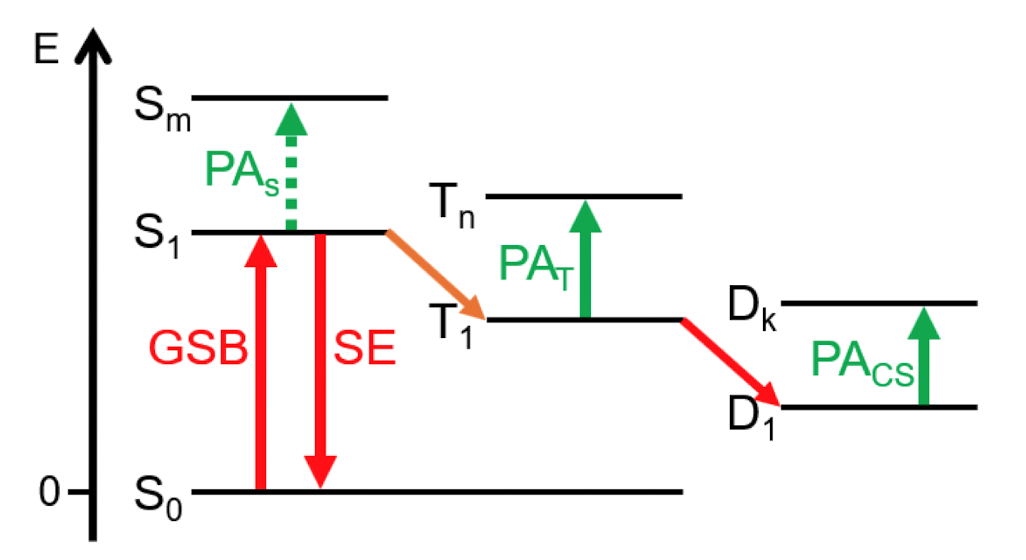
\includegraphics[width = 0.6\textwidth]{Pictures/Transient-Absorption.png}
    \captionof{figure}{
        Ground state bleaching (GSB), stimulated emission (SE) and photoinduced absorption (PA) of different states. \cite{Kilchert.04.2023}
    }
    \label{fig:transient}
\end{center}

In the transient absorption spectroscopy gets the excited singlet state occupied by the stimulation by an excitation pulse (pump laser). With a fast ISC, the molecules in the triplet state can be further excited by a second excitation pulse (probe laser), which is weaker than the pulse of the pump laser. The absorption of this second pulse is proportional to the occupation of the triplet state. By varying the time interval between the two pulses (time delay), a time-resolved transient absorption spectrum can be obtained. This delayed pulse interacts with the matter in its excited state. The interaction of the delayed pulse with the material leads to three observable effects in the spectrum: 
\begin{itemize}
    \item \textbf{Ground State bleaching} (GSB),
    \item \textbf{transient absorption} (TA),
    \item \textbf{stimulated emission} (SE).
\end{itemize}
Ground state bleaching occurs because of the excitation process due to the lowered ground-state density, which can absorb less light. Transient absorption spectroscopy gives insight into energy transfer and charge transfer dynamics of the material systems. To make the mentioned effects visible, the intensity of the pump laser has to be sufficiently large. \cite{JulienFrancoisGorenflot.2015}
In transient absorption spectroscopy occurs signals which are negative and positive. Negative signals are connceted to the absorption of the ground state, whereas positive signals are correlated to the absorption of the exited state. \cite{Kennis.2009}

\section{Incluence of Polarization on Transient Absorption Spectroscopy}
\label{sec:polLight}

As laser light is often polarized, polarization effects can occur during the experiment. The effect happens because the absorption is sensitive to the position of the transition dipole moment to the electric field. This leads to a photon selection in the absorption. In the case of the experiment this effect is not important as probing happens on the scale of nanometers, when the vibration of the molecule is in the range of picoseconds.